\documentclass{article}%
\usepackage[T1]{fontenc}%
\usepackage[utf8]{inputenc}%
\usepackage{lmodern}%
\usepackage{textcomp}%
\usepackage{lastpage}%
\usepackage{geometry}%
\geometry{tmargin=1cm,lmargin=1cm}%
\usepackage{amsmath}%
\usepackage{tikz}%
\usepackage{pgfplots}%
\pgfplotsset{compat=newest}%
%
%
%
\begin{document}%
\normalsize%
\section{Quick Scan Survey: first survey in the app}%
\label{sec:QuickScanSurveyfirstsurveyintheapp}%
This document contains the results of the survey conducted on: 2021{-}06{-}23 15:27:19. %
You can find the questions and their results below.         Please be aware that this document generation system         is in early stages, it is possible for items to not fit pages properly             or other odd things to happen.%
\newline%
%
1: Is de winkel goed bereikbaar met het openbaar vervoer? %
\newline%
%
\newline%
%
   True%
\newline%
%
2: Is er voldoende parkeergelegenheid bij de winkel? %
\newline%
%
\newline%
%
3: Zijn er alternatieve verkooppunten in de omgeving met vergelijkbare producten of diensten? %
\newline%
%
\newline%
%
   False%
\newline%
%
4: Wordt de klant begroet bij binnenkomst? %
\newline%
%
\newline%
%
5: Welke manier van prijscommunicatie (schapkaartjes, stickers, etc.) worden er gebruikt? %
\newline%
%
\newline%
%
6: Hoe wordt er afgeprijsd? (Handmatig? Of met ESLs?). %
\newline%
%
\newline%
%
7: Is er additionele productinformatie beschikbaar? %
\newline%
%
\newline%
%
   True%
\newline%
%
8: Zijn er IT oplossingen ingezet om klanten te ondersteunen in hun koopproces? %
\newline%
%
\newline%
%
   True%
\newline%
%
9: Wat is het THT beleid? %
\newline%
%
\newline%
%
10: Worden er schapwissels regelmatig doorgevoerd? %
\newline%
%
\newline%
%
11: Hoe vaak wordt het filiaal beleverd, en hoe vaak wordt de levering aangevuld? %
\newline%
%
\newline%
%
12: Hoe wordt het personeel ingeroosterd? Wordt er een WFM tool gebruikt, of gebeurt dit handmatig? %
\newline%
%
\newline%
%
13: Wat is het ziekteverzuimpercentage? %
\newline%
%
\newline%
%
14: Welke betaalmogelijkheden zijn er? %
\newline%
%
\newline%
%
15: Is het mogelijk om producten in de winkel te retourneren? %
\newline%
%
\newline%
%
   False%
\newline%
%
16: Is er een webshop beschikbaar? %
\newline%
%
\newline%
%
   True%
\newline%
%
17: Kunnen online gekochte producten in de winkel gerouterneerd worden? %
\newline%
%
\newline%
%
   True%
\subsection{Table of something}%
\label{subsec:Tableofsomething}%
\begin{tabular}{rc|cl}%
\hline%
1&2&3&4\\%
\cline{1%
-%
2}%
&&&\\%
4&5&6&7\\%
\end{tabular}

%
\section{The fancy stuff}%
\label{sec:Thefancystuff}%
\subsection{Correct matrix equations}%
\label{subsec:Correctmatrixequations}%
\[%
\begin{pmatrix}%
2&3&4\\%
0&0&1\\%
0&0&2%
\end{pmatrix} \begin{pmatrix}%
100\\%
10\\%
20%
\end{pmatrix} = \begin{pmatrix}%
310\\%
20\\%
40%
\end{pmatrix}%
\]

%
\subsection{Alignat math environment}%
\label{subsec:Alignatmathenvironment}%
\begin{alignat*}{2}%
\frac{a}{b} &= 0 \\%
\begin{pmatrix}%
2&3&4\\%
0&0&1\\%
0&0&2%
\end{pmatrix}%
\begin{pmatrix}%
100\\%
10\\%
20%
\end{pmatrix}%
&=%
\begin{pmatrix}%
310\\%
20\\%
40%
\end{pmatrix}%
\end{alignat*}

%
\subsection{Beautiful graphs}%
\label{subsec:Beautifulgraphs}%
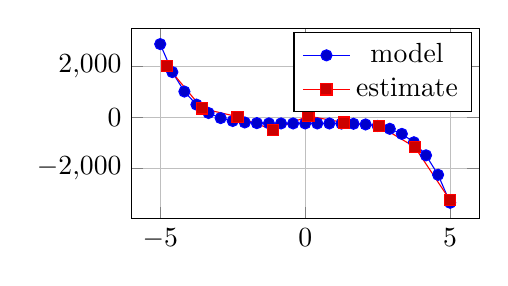
\begin{tikzpicture}%
\begin{axis}[height=4cm, width=6cm, grid=major]%
\addplot{-x^5 - 242};%
%
\addlegendentry{model}%
\addplot coordinates {%
(-4.77778,2027.60977)%
(-3.55556,347.84069)%
(-2.33333,22.58953)%
(-1.11111,-493.50066)%
(0.11111,46.66082)%
(1.33333,-205.56286)%
(2.55556,-341.40638)%
(3.77778,-1169.2478)%
(5.0,-3269.56775)%
};%
%
\addlegendentry{estimate}%
\end{axis}%
\end{tikzpicture}

%
\end{document}